\chapter{\sffamily Managing a rugby match}

{\bfseries\sffamily Concept.} Building a toy model simulation of a rugby match whose outcome can be manipulated through correctly-timed player substitutions and game management decisions. The dexetera state manipulation framework we have built around the stochadex can meet these requirements, and a dashboard can be created for user interaction. All this combines together to make a simple dashboard game, which we call: `trywizard'. For the mathematically-inclined, this chapter will motivate the construction of a specific modelling framework for rugby match simulation. For the programmers, the public Git repository for the code described in this chapter can be found here: \href{https://github.com/umbralcalc/trywizard}{https://github.com/umbralcalc/trywizard}.

\section{\sffamily Designing the event simulation engine}

Since the basic state manipulation framework and simulation engine will run using \href{https://github.com/umbralcalc/dexetera}{dexetera}, the mathematical novelties in this project are all in the design of the rugby match model itself. And, as ever, we're not especially keen on spending a lot of time doing detailed data analysis to come up with the most realistic values for the parameters that are dreamed up here. Even though this would also be interesting.\footnote{One could do this data analysis, for instance, by scraping player-level performance data from one of the excellent websites that collect live commentary data such as \href{https://www.rugbypass.com/}{rugbypass.com} or \href{https://www.espn.co.uk/rugby/}{espn.co.uk/rugby}.}

We need to begin by specifying an appropriate event space to live in when simulating a rugby match. It is important at this level that events are defined in quite broadly applicable terms, as it will define the state space available to our stochastic sampler and hence the simulated game will never be allowed to exist outside of it. So, in order to capture the fully detailed range of events that are possible in a real-world match, we will need to be a little imaginative in how we define certain gameplay elements when we move through the space.

The diagrams below sum up what should hopefully work as a decent initial approximation while providing a little context with specific examples of play action.

\begin{figure}[h]
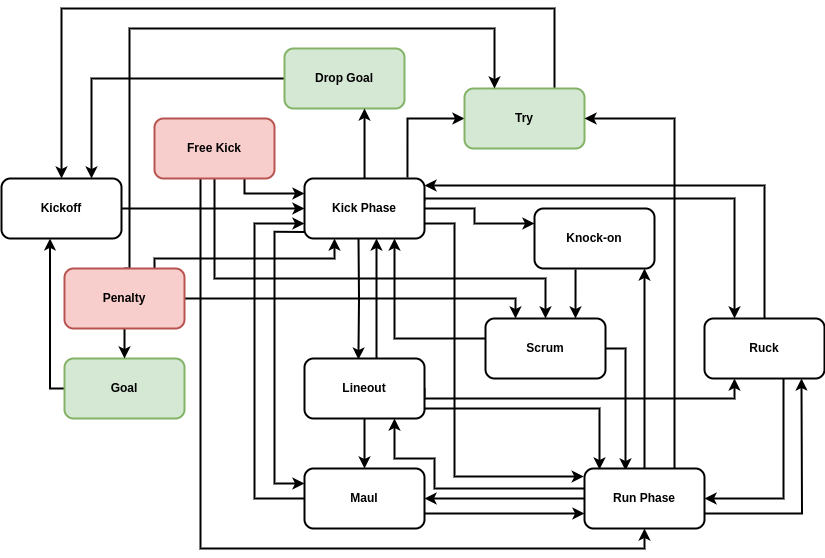
\includegraphics[width=14cm]{images/trywizard-event-graph.drawio.png}
\caption{Simplified event graph of a rugby union match.}
\label{fig:event-graph}
\end{figure}

\section{\sffamily Linking to player attributes}

\section{\sffamily Deciding on gameplay actions}

\section{\sffamily Writing the game itself}